% -*- coding: utf-8; mode: latex; -*-

% +++
% latex = "lualatex"
% +++

%
% FIT2023 向け LaTeX クラスファイル
% https://github.com/trueroad/FITpaper-class
%
% サンプルファイル
%
% Copyright (C) 2018, 2019, 2022, 2023 Masamichi Hosoda.
% All rights reserved.
%

\documentclass{FITpaper}

% 図の貼り込み用
\usepackage{graphicx}

% 最終ページで両カラムの下端を揃える
%\usepackage[balance]{nidanfloat}
\usepackage{flushend}
\def\BibTeX{{\rm B\kern-.05em{\sc i\kern-.025em b}\kern-.08em
    T\kern-.1667em\lower.7ex\hbox{E}\kern-.125emX}}
% 和文タイトル
\jtitle{ブラウザ上でユーザが編集可能な言語パターンマッチシステムの構築 }

% 欧文タイトル
\etitle{Building a user-editable language pattern matching system in the browser}

% 著者数:著者の数だけ c を書く
\authors{cc}

% 和文著者名:著者名間に & を書く
% 所属番号を \affmark でつける
\jauthors{%
  桂 辰弥\affmark{1} &
  竹内 孔一\affmark{1}
}

% 欧文著者名:著者名間に & を書く
\eauthors{%
  Tatsuya Katsura &
  Koichi Takeuchi
}

% 所属
% \affmark でつけた番号毎に指定
\afftext{1}{岡山大学}


\begin{document}

\maketitle

\section{はじめに}
テキスト中の特定のフレーズや表現を見つけることは,言語および教育分野において必要となることがある.テキストデータから特定のキーワードやフレーズの出現位置や文脈を抽出するためのプログラムとしてコンコーダンサがある.コンコーダンサは語学学習において特定のフレーズや表現の使用例を実際の文脈で把握することで,語彙や文法の理解、単語の使用法や文脈の把握に役立ち,学習者の語彙や表現力の向上に役立つ.
パターンマッチングはテキストの表層で検索を行う正規表現とは異なり,情報を抽出したい文を対象に予め関係する文や文の一部に対応する文構造のパターンを用意し,そのパターンに合致する結果を取得するものである.
有名なコンコーダンサの例として,Sketch Engineがある.Sketch Engine\footnote{https://www.sketchengine.eu/},はクエリ言語としてCQL(Corpus Query Language)\footnote{https://www.sketchengine.eu/documentation/corpus-querying/}が使用されており,コーパス内で正規表現や演算子を組み合わせることでパターンマッチを行うことができる.
しかしSketch Engineは,コーパスベースの言語分析や統計的な情報抽出が主な役割であるため,
テキスト中から依存関係解析を持つ表現を抽出する際には前処理が必要となる.

ユーザ自らがこれらを考慮してテキスト中の特定フレーズや表現を抽出するようなシステムを構築することは容易ではない.そこで本研究では解析モジュールで解析した結果をユーザ自身が求める表現をあらかじめ用意された検索ブロックで組み合わせてシステムに投入し,事例を検索できるシステムの開発を行っている.先行研究 においてWEBアプリケーションとしてJavaScriptとPythonを利用した基本システムを構築したが,
システムの本格利用にはいくつかの課題が残されている.そこで本報告では検索エンジンの中心部分であるPrologデータベースの実装の改良,および、大規模なテキストが扱えるためにデータベースをシステムに導入したので、この改良について報告する.


\section{提案する言語パターンマッチシステム}
本章では提案する言語パターンマッチシステムを構築している環境についての概要と処理の流れについて述べる.
\begin{figure}[htbp]
  \centering
  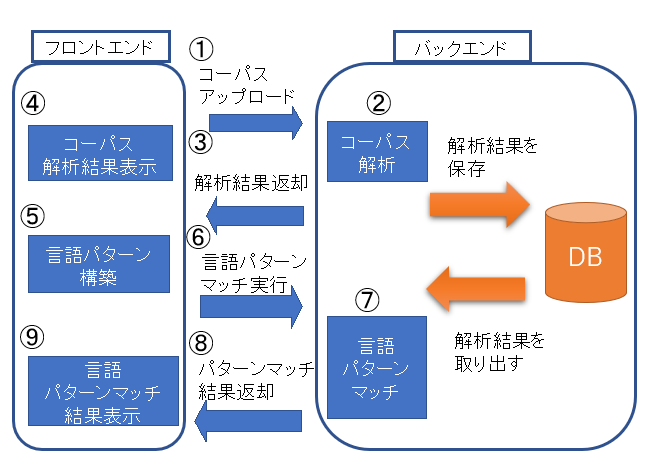
\includegraphics[scale=0.4]{fig/system_fig.png}
  \caption{システムの構成図}
  \label{fig:sys}
\end{figure}
\subsection{言語パターンマッチシステムの概要}
本システムは図\ref{fig:sys}のようにユーザが視覚的に操作を行うフロントエンドシステムとユーザが要求したテキストの処理バックエンドシステムに切り分けて構成している.
フロントエンドシステムはJavascriptのライブラリであるReact.jsで構成されており
主な機能としてはテキストファイルのアップロード,検索する言語パターンの構築,解析結果の表示,検索結果の表示などがある.

バックエンドシステムはPythonのWebフレームワークであるDjangoとデータベースシステムであるElasticsearchで構成されており,
主な機能としてはテキストファイルの解析,ユーザが構築した検索クエリの言語パターンマッチ実行などがある.

詳しい処理の流れについては以降の節で述べる.

\subsection{処理の流れについて}
バックエンドで行われるテキスト解析,言語パターンマッチ実行の際の処理の流れについてそれぞれ説明する.

テキストの解析の処理はユーザがアップロードしたテキストファイルの文にASA{}を用いて形態素解析,係り受け解析,項構造解析を適応させる.解析した結果の文の木構造を図\ref{fig:tree}に示す.
その後Prolog述語に変換を行い,データベースに保存する.変換するProlog述語は以下の表\ref{tbl:predicates}ように定義しており.図\ref{fig:prolog}のように変換される.
言語パターンマッチの処理はユーザが構築した検索パターンを送信し,データベースから各文に対応するPrologを取得し,Prologパターンマッチを実行する.
パターンマッチを実行するProlog処理系としてSWI-Prologのpythonモジュールであるpyswipを使用している.


\begin{figure}[htbp]
  \centering
  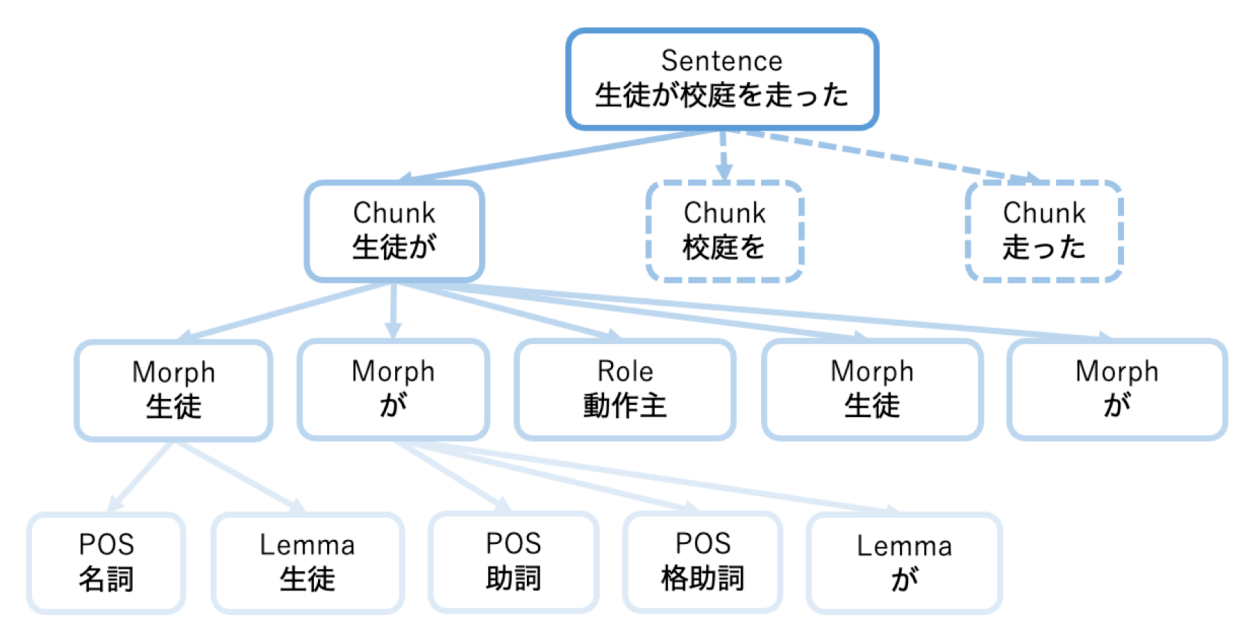
\includegraphics[scale=0.4]{fig/tree.eps}
  \caption{文を解析した木構造の例}
  \label{fig:tree}
\end{figure}
\begin{table}[htbp]
  \caption{Prologの述語一覧}
  {\small
  \begin{center}
    \begin{tabular}{|l||l|l|}\hline
      述語                         &  第2引数   & 第3引数               \\
      \hline 

      chunk(SENTENCE\_ID, 0,\_)           &  根ノード ID& 文節 ID                   \\
      morph(SENTENCE\_ID, \_, \_)      & 文節 ID& 形態素 ID                \\
      main(SENTENCE\_ID, \_, \_)         &文節 ID & 主形態素 \\
      part(SENTENCE\_ID, \_, \_)         &文節 ID& 副形態素\\
      role(SENTENCE\_ID, \_, \_)         &文節 ID& 意味役割  \\
      semantic(SENTENCE\_ID, \_, \_)     &文節 ID & 概念\\
      surf(SENTENCE\_ID, \_, \_)          &ノード ID& ノードの表層\\               
      surfBF(SENTENCE\_ID, \_, \_)       &形態素 ID& 形態素の基本形        \\
      sloc(SENTENCE\_ID, \_, \_)&文節/形態素 ID & 出現位置\\
      pos(SENTENCE\_ID, \_, \_)          &形態素 ID& 品詞\\                                        
      dep(SENTENCE\_ID, \_, \_)        &文節 ID & 文節 ID\\
        \hline
    \end{tabular}
  
    \label{tbl:predicates}
  \end{center}
  }
\end{table}
\begin{figure}[htbp]
  \centering
  \includegraphics[scale=0.5]{fig/prolog_data.png}
  \caption{システムの構成図}
  \label{fig:prolog}
\end{figure}

次に
\section{評価実験}

\subsection{実験内容}
\subsection{結果}
\begin{table}[htbp]
  \centering
    \caption{パターンマッチの検索時間(秒)}
    \label{pattern_result}
    \begin{tabular}{|l||r|r|}  
      \hline
      文の数 & 検索時間\\ \hline \hline
      1 & 0.110\\\hline
      10 &  0.531\\\hline
      100 & 5.54\\ \hline
      1000 &  60 \\\hline
      5000 &  312\\\hline
      10000 &  620\\ \hline
    \end{tabular}
  \end{table}
\section{考察と結論}

\acknowledgment{%
  謝辞の文章を\texttt{\textbackslash acknowledgment}で指定します。
  使わなければ謝辞は出力されません。
}

%\bibliographystyle{unsrt}

%\bibliography{all,my-results}


\end{document}